%\documentclass[varwidth,border=10pt]{standalone}
\documentclass[aps,pra,twocolumn,superscriptaddress]{revtex4-1} %reprint
\thispagestyle{empty}
%\usepackage{subcaption}
%\usepackage[labelformat=parens,labelsep=quad, skip=3pt]{caption}
\usepackage{etex}
\usepackage{amsmath}
\usepackage{bm}
\usepackage{bbm}
\usepackage{listings}
% % \textwidth 16cm \textheight 23.5cm
% \renewcommand{\baselinestretch}{1.2}
\usepackage{graphicx}
\usepackage{graphics}
\usepackage{epsfig}
\usepackage{color}
\usepackage[dvipsnames]{xcolor}
\usepackage{multirow}
\usepackage[colorlinks]{hyperref}
\usepackage{fancyhdr}
\usepackage{calc}
\usepackage{natbib} %[numbers]
\usepackage{bibentry}
\usepackage{bbm}
\usepackage{bbold}

% todo list and commands
%\usepackage{todonotes}
%% to avoid the conflict with amths package % not working
%\makeatletter
%\providecommand\@dotsep{5}
%\makeatother
%\listoftodos\relax
%\usepackage{makeidx}
%\allowdisplaybreaks
%% for eps transfering to pdf.
%\usepackage[update,prepend]{epstopdf}
%\usepackage{ifpdf}
%
%\ifpdf
%   \usepackage{graphicx}
%   \usepackage{epstopdf}
%   \epstopdfsetup{suffix=}
%   \DeclareGraphicsRule{.eps}{pdf}{.pdf}{`epstopdf #1}
%   \pdfcompresslevel=9
%\else
%   \usepackage{graphicx}
%\fi
% subfig
\usepackage{mwe}
\usepackage[caption=false]{subfig}
% to fix a figure's position using [H] option of thec figure.
\usepackage{float}
% to use \lesssim and other math symbols
%\usepackage{amssymb}
% set package options
\captionsetup[subfloat]{position=top,singlelinecheck=off,labelfont={normalsize,sf}, %justification=raggedright,
  labelformat=simple,listofformat=subparens,aboveskip=0pt,parskip=0pt,farskip=5pt,
  captionskip=0pt}

% customize subfigure label to capitals
\renewcommand{\thesubfigure}{(\alph{subfigure})}
  
  %==== scattering and optical pumping rates ====%
  \newcommand{\gammauu}{\gamma_{\uparrow \rightarrow \uparrow}}
  \newcommand{\gammadd}{\gamma_{\downarrow \rightarrow \downarrow}}
  \newcommand{\gammaud}{\gamma_{\uparrow \rightarrow \downarrow}}
  \newcommand{\gammadu}{\gamma_{\downarrow \rightarrow \uparrow}}
  \newcommand{\gammau}{\gamma_{\uparrow}}
  \newcommand{\gammad}{\gamma_{\downarrow}}
  
  %==== effective areas ======
  \newcommand{\Ain}{A_{\rm in}}
  \newcommand{\Abir}{A_N}
  \newcommand{\AF}{A_{\rm Far}} % for the Faraday protocol.
  \newcommand{\Ai}{A_{\rm in}} % for the input light.
  \newcommand{\Aint}{A_{\rm int}} % for the interaction area.
  
\begin{document}
\begin{figure}[htb]
\centering
 \begin{minipage}[h]{\linewidth}
 %\begin{tabular}{*{2}{b{0.2\textwidth-2\tabcolsep}}}
  \subfloat[h][]{
    %% This file was created by matlab2tikz.
%
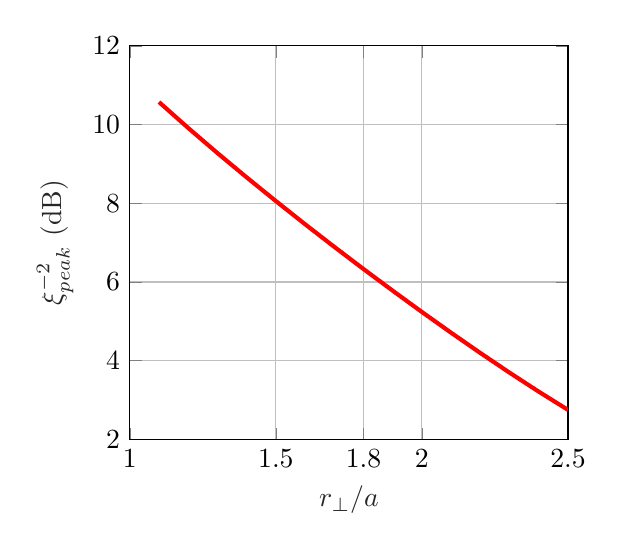
\begin{tikzpicture}

\begin{axis}[%
width=5.565cm,
height=5cm,
at={(0cm,0cm)},
scale only axis,
xmin=1.0000,
xmax=2.5000,
xtick={1.0000,1.5000,1.8000,2.0000,2.5000},
xlabel style={font=\color{white!15!black}},
xlabel={$r_\perp/a$},
ymin=2.0000,
ymax=12.0000,
ylabel style={font=\color{white!15!black}},
ylabel={$\xi^{-2}_{peak}$ (dB)},
axis background/.style={fill=white},
xmajorgrids,
ymajorgrids
]
\addplot [color=red, line width=1.5pt, forget plot]
  table[row sep=crcr]{%
1.1000	10.5712\\
1.2000	9.9128\\
1.3000	9.2762\\
1.4000	8.6588\\
1.5000	8.0571\\
1.6000	7.4685\\
1.7000	6.8935\\
1.8000	6.3307\\
1.9000	5.7799\\
2.0000	5.2394\\
2.1000	4.7118\\
2.2000	4.1974\\
2.3000	3.6980\\
2.4000	3.2157\\
2.5000	2.7531\\
};
\end{axis}
\end{tikzpicture}%
    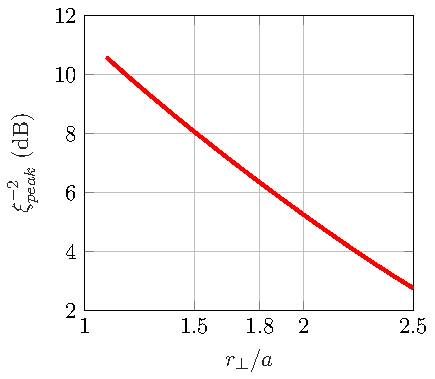
\includegraphics[width=0.45\linewidth]{../Fig7a}
    }
    \hfill
  \subfloat[h][]{
      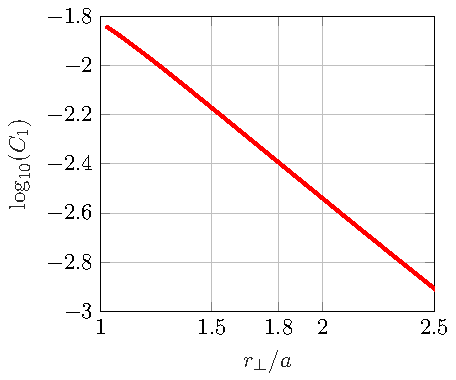
\includegraphics[width=0.48\linewidth]{../Fig7b}
      %% This file was created by matlab2tikz.
%
%The latest updates can be retrieved from
%  http://www.mathworks.com/matlabcentral/fileexchange/22022-matlab2tikz-matlab2tikz
%where you can also make suggestions and rate matlab2tikz.
%
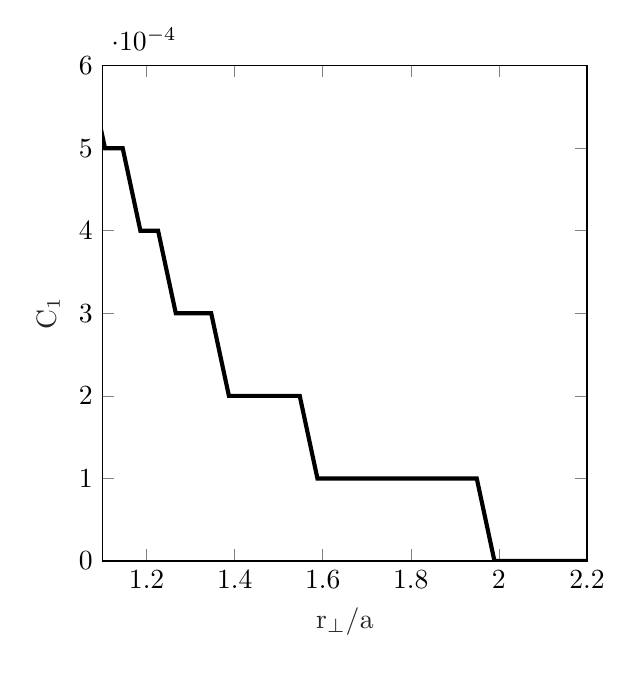
\begin{tikzpicture}

\begin{axis}[%
width=2.422in,
height=2.477in,
at={(0.406in,0.413in)},
scale only axis,
xmin=1.1000,
xmax=2.2000,
xlabel style={font=\color{white!15!black}},
xlabel={$\text{r}_\perp\text{/a}$},
ymin=0.0000,
ymax=0.0006,
ylabel style={font=\color{white!15!black}},
ylabel={$\text{C}_\text{1}$},
axis background/.style={fill=white}
]
\addplot [color=black, line width=1.5pt, forget plot]
  table[row sep=crcr]{%
1.0653	0.0006\\
1.1055	0.0005\\
1.1457	0.0005\\
1.1859	0.0004\\
1.2261	0.0004\\
1.2663	0.0003\\
1.3065	0.0003\\
1.3467	0.0003\\
1.3869	0.0002\\
1.4271	0.0002\\
1.4673	0.0002\\
1.5075	0.0002\\
1.5477	0.0002\\
1.5879	0.0001\\
1.6281	0.0001\\
1.6683	0.0001\\
1.7085	0.0001\\
1.7487	0.0001\\
1.7889	0.0001\\
1.8291	0.0001\\
1.8693	0.0001\\
1.9095	0.0001\\
1.9497	0.0001\\
1.9899	0.0000\\
2.0302	0.0000\\
2.0704	0.0000\\
2.1106	0.0000\\
2.1508	0.0000\\
2.2312	0.0000\\
};
\end{axis}
\end{tikzpicture}%
      }
   \end{minipage}\vfill
   \begin{minipage}[h]{\linewidth}
    %\begin{tabular}{*{2}{b{0.2\textwidth-2\tabcolsep}}}
     \subfloat[h][]{
       %\input{fig/square waveguide_peakxi_rp_NA2500.tex}
       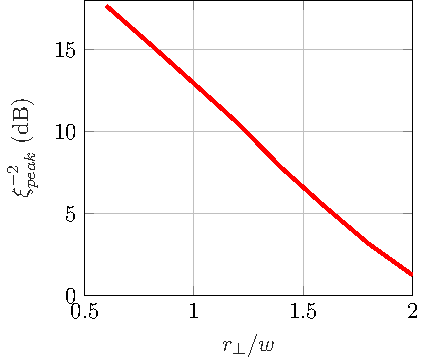
\includegraphics[width=0.45\linewidth]{../Fig7c}
       }
       \hfill
     \subfloat[h][]{\vspace{-8px}
         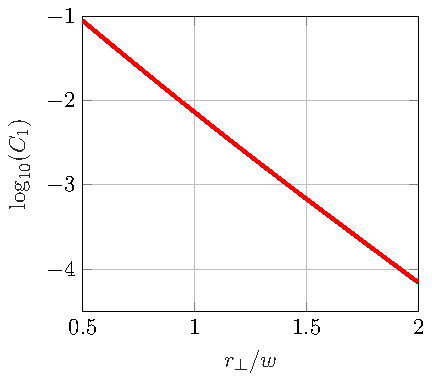
\includegraphics[width=0.46\linewidth]{../Fig7d}
         %\input{fig/square waveguide_C1_y.tex}
         }
   \end{minipage}
\end{figure}
\end{document}